\documentclass[12pt,fleqn]{article}\usepackage{../../common}
\begin{document}
Da�lar Aras�nda En Optimal Y�r�y�� Yolu Bulmak

\begin{minted}[fontsize=\footnotesize]{python}
from mpl_toolkits.mplot3d import Axes3D
from scipy.spatial.distance import cdist
from matplotlib import cm

def func(x, y):
    s1 = 2.2; x1 = 2.0; y1 = 2.0
    g1 = np.exp( -4 *np.log(2) * ((x-x1)**2+(y-y1)**2) / s1**2)
    return g1 

D = 50

x = np.linspace(0,5,D)
y = np.linspace(0,5,D)

xx,yy = np.meshgrid(x,y)
zz = func(xx,yy)

fig = plt.figure()
ax = fig.gca(projection='3d')
ax.set_xlim(0,5)
ax.set_ylim(0,5)
surf = ax.plot_wireframe(xx, yy, zz,rstride=10, cstride=10)

t = np.linspace(0,1.0,100)

a1,a2,a3 = 1.5, 10.1, 4.0
b1,b2,b3 = 0.3, 0.4, 30.3

sx,sy=(1.0,1.0)
ex,ey=(0.3,4.0)

a4 = ex - sx - (a1+a2+a3)
b4 = ey - sy - (b1+b2+b3)

x = 1.0 + a1*t + a2*t**2 + a3*t**3 + a4*t**4 
y = 1.0 + b1*t + b2*t**2 + b3*t**3 + b4*t**4

ax.plot3D(x, y, func(x,y),'r.')

plt.savefig('calc_multi_40_elev_01.png')
\end{minted}

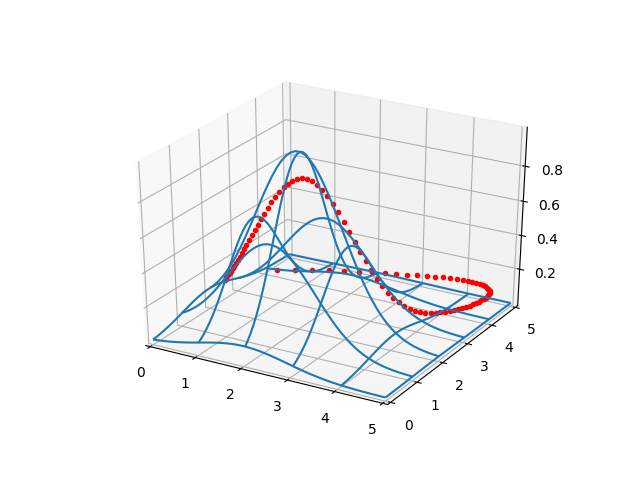
\includegraphics[width=20em]{calc_multi_40_elev_01.png}






[devam edecek]

\end{document}
